\documentclass{article}
\usepackage[T1]{fontenc}
\usepackage{lmodern}
\usepackage{graphicx}
\usepackage{amsmath,amssymb}
\usepackage[a4paper,margin=2cm]{geometry}
\usepackage[absolute,overlay]{textpos}
\setlength{\TPHorizModule}{1mm}
\setlength{\TPVertModule}{1mm}
\usepackage[indonesian]{babel}
\usepackage{hyperref}
\setlength{\emergencystretch}{2em}
% unit: Halaman 55

\begin{document}

% === Halaman 55 (llm) ===

\section*{Contoh substitusi di dalam block cipher AES:}

\vspace{60mm}

\noindent Input: 23 (Hexadecimal)\\
Output: 26 (Hexadecimal)

\noindent Cara substitusi;\begin{itemize}
    \item Cari perpotongan baris 2 dengan kolom 3
    \item hasilnya adalah 26
\end{itemize}

% deskripsi: Tabel substitusi (S-Box) untuk AES yang berisi nilai-nilai hexadecimal dalam grid 16x16.
% bbox normalisasi: [0.0000, 0.1600, 0.6800, 0.7700]
\begin{textblock*}{142.80mm}(0.00mm,47.52mm)
\noindent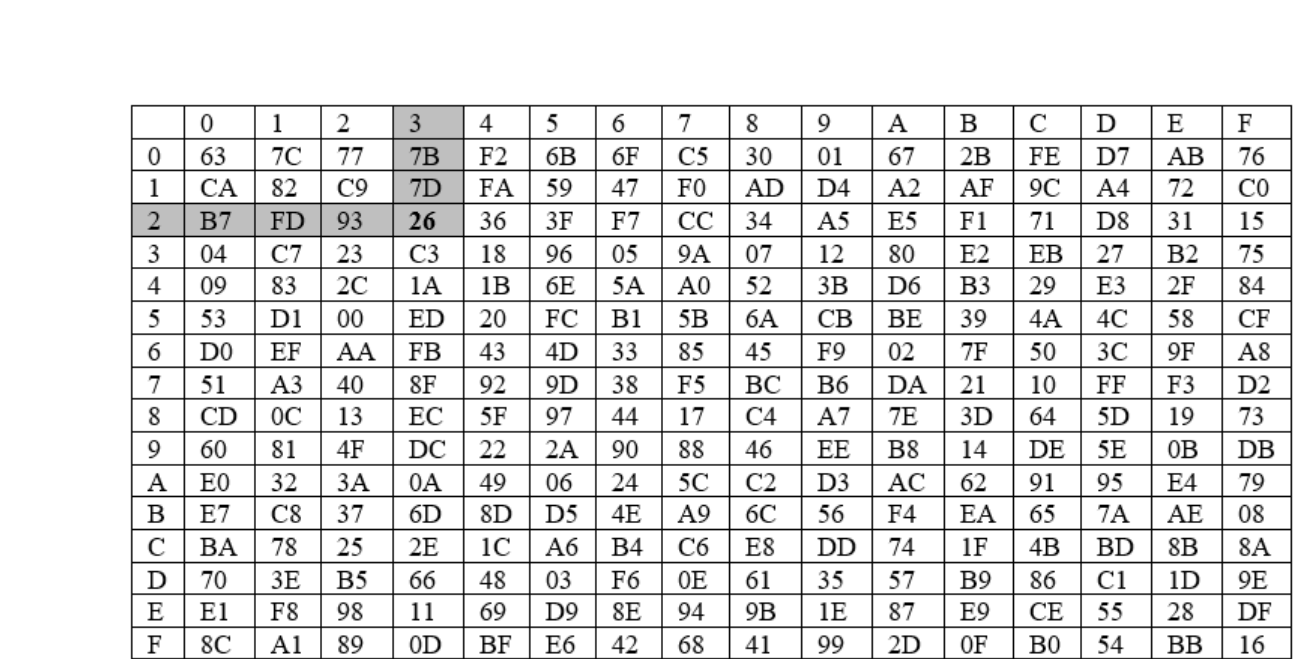
\includegraphics[width=142.80mm,height=181.17mm]{../../images/llm/page_055_img_01.png}%
\end{textblock*}

\end{document}
